%!TeX root=../tese.tex
%("dica" para o editor de texto: este arquivo é parte de um documento maior)
% para saber mais: https://tex.stackexchange.com/q/78101/183146

%% ------------------------------------------------------------------------- %%


% Recomendação Will: mudar nome do cap para método de avaliação do algoritmo ou similar: X

% ao invés de usar delineamento usar design ou desenho: X

% colocar uma tabela ou imagem ilustrando o uso do quadrado latino no nosso trabalho: 

% colocar nota de rodapé em desenvolvimento primeiro paragrafo referente a ultimo acesso e URL site:X

% WILL : "Qual a diferença de atributos entre os diferentes tanques e torres mesmo? Acho que vocês mencionam antes no texto mas é bom repetir, mover para aqui, ou pelo menos referenciar a seção onde foi dito": X

% Mencionar figuras no texto: X

% Mencionar Tabelas no texto: X

% deixar mais claro que soluções ingenuas servem para ser comparadas com algoritmo genético.: X

% Figuras sempre com letra maiúscula quando for mencionar no texto:X



\chapter{Método de Avaliação do algoritmo}
\label{cap:testes}

Com o algoritmo funcional, foi necessário buscar maneiras de avaliar seu desempenho para garantir sua eficiência \textit{versus} inimigos gerados aleatoriamente. Foram consideradas as possibilidades de distribuir os jogos e coletar \textit{feedback} de outros jogadores, mas considerando possíveis avaliações subjetivas para os jogos relativamente simples e limitações de tempo decidiu-se por utilizar métodos automatizados para coleta de resultados de dano em sequências de ondas.

%% ------------------------------------------------------------------------- %%
\section{Metodologia}
\label{sec:t-metodologia}

Segundo o Teorema Central do Limite, são necessárias, no mínimo, 30 amostras para que a média das mesmas tenha uma distribuição aproximadamente normal \citep{Magalhaes_estatistica}. Portanto, foram planejados experimentos nos jogos para geração de 30 amostras de dados em cada modo de jogo, para produção de gráficos com o comportamento das ondas, e desenho em quadrado latino.

%% ------------------------------------------------------------------------- %%
\subsection{Quadrado Latino}
\label{sec:t-quad-latino}

A coleta e disposição dos dados teve como objetivo a montagem de um quadrado latino.
Um quadrado latino de v linhas por v colunas é um arranjo de v letras latinas na forma de uma tabela, de maneira que cada letra ocorra apenas uma vez em cada linha, e uma vez em uma coluna, \citep{Design_exp_latin_sq}. Por exemplo, a tabela 3 x 3 é um quadrado latino:

\begin{table}
\caption{Exemplo de quadrado latino}
\begin{tabular}{ccc}
    A       & B    & C     \\ 
    B       & C    & A     \\
    C       & A    & B      \\
\end{tabular}
\end{table}

O desenho em quadrado latino é usado em experimentos onde os objetos de estudo estão submetidos a uma series de tratamentos, onde o tempo decorrido terá influência significativa nas respostas \citep{Design_exp_latin_sq}. A escolha do desenho em quadrado latino também é apropriada dado que os ambientes em que os testes foram feitos não são exatamente iguais, e por existirem dois fatores que podem influenciar nas respostas\citep{campbell:quadradolatino} - a inteligência artifical e o jogador que está sendo simulado.


%% ------------------------------------------------------------------------- %%
\section{Experimentos com o Algoritmo}
\label{sec:t-testes-algoritmo}

Durante o decorrer dos experimentos, notou-se incoerências nos testes realizados pelos códigos produzidos. Em especial, na função \textit{fitness} e na taxa de mutação.

\subsection{Fitness}

A função de avaliação (\textit{fitness}) é passada pelo usuário do código e, portanto, tiveram que ser criadas. No próximo capítulo \ref{sec:a-fitness}, será explicado mais detalhadamente sobre os resultados produzidos com diferentes funções de avaliação (\textit{fitness}) e as tentativas de alcançar outros resultados com base nelas.

\subsection{Taxa de mutação}

A taxa de mutação também pode ser definida pelo  usuário. Em particular, para testes pequenos como os feitos neste trabalho, é recomendado um valor entre $5\%$ até $20\%$. \citep{haupt00:mutationprob}.

Uma diferente abordagem ainda nesse tópico, é a utilização de taxas de mutação que decrescem conforme o tempo. Possui seus benefícios em testes de natureza mais determinística, já que espera-se que o algoritmo chegue em um ponto de convergência nas populações finais. Este método proporciona maior \textit{exploration} nas gerações iniciais, uma vez que está buscando o melhor resultado sem se prender em pontos de máximo local e maior \textit{exploitation} nas gerações finais, pois estará explorando o melhor resultado que obteve até o momento. \citep{eiben98:exploitvsexplore}

%% ------------------------------------------------------------------------- %%
\section{Desenvolvimento}
\label{sec:t-desenvolvimento}

Para fazer a coleta dos dados de maneira mais eficiente, os jogos foram adaptados para armazenarem os resultados das ondas. Foram desenvolvidas cenas no \textit{Godot} (menus e fases de teste), como pode se ver nas Figuras \ref{fig:tela-de-teste-tower defense} e \ref{fig:tela-de-teste-space-shooter}, que executam os testes de maneira determinística e consistente, sem aceitar \textit{input} do jogador. O botão \textit{Test Mode} acessa a interface de testes, enquanto o botão \textit{Play Defaut mode} utiliza o modo de jogo padrão. Todos os resultados são gravados em arquivos ".txt" com nome e formatação pré-definidos para facilitar a análise exploratória dos dados em \textit{Jupyter Notebook} \footnote{ \url{https://github.com/raktanaka/tcc-results} - 21/12/2021}.

\pagebreak

\begin{figure}
  \centering
  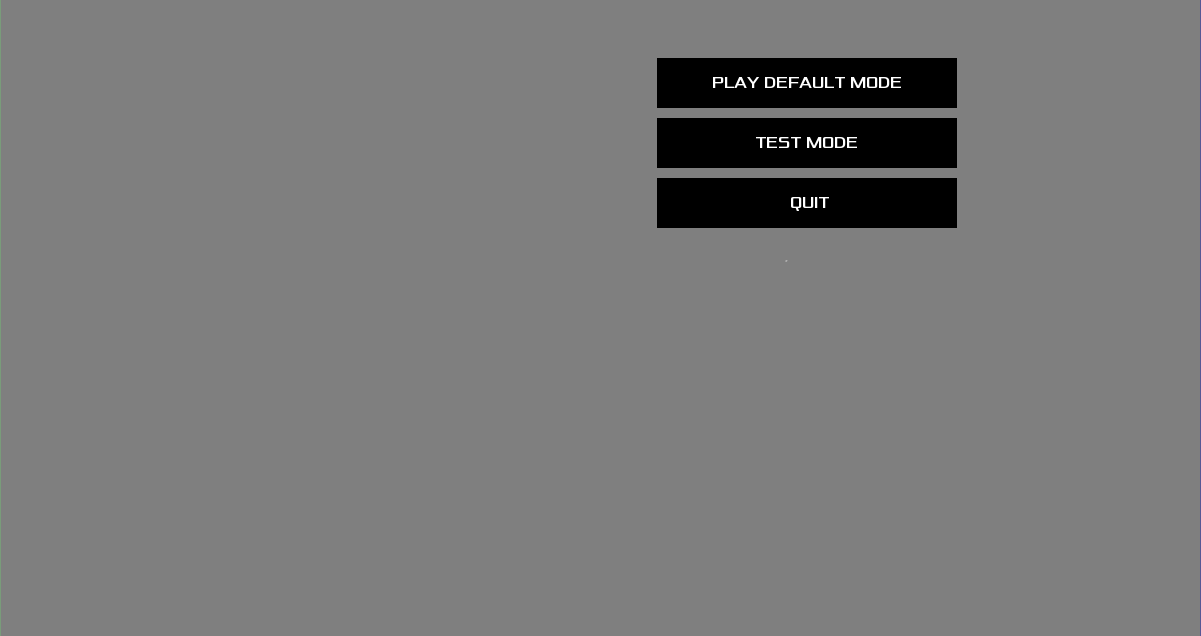
\includegraphics[width=.8\textwidth]{td/Tela_Teste_TDD.png}
  \caption{Tela de Teste Tower defense. Imagem retirada do próprio jogo.\label{fig:tela-de-teste-tower defense}}
\end{figure}

\begin{figure}
  \centering
  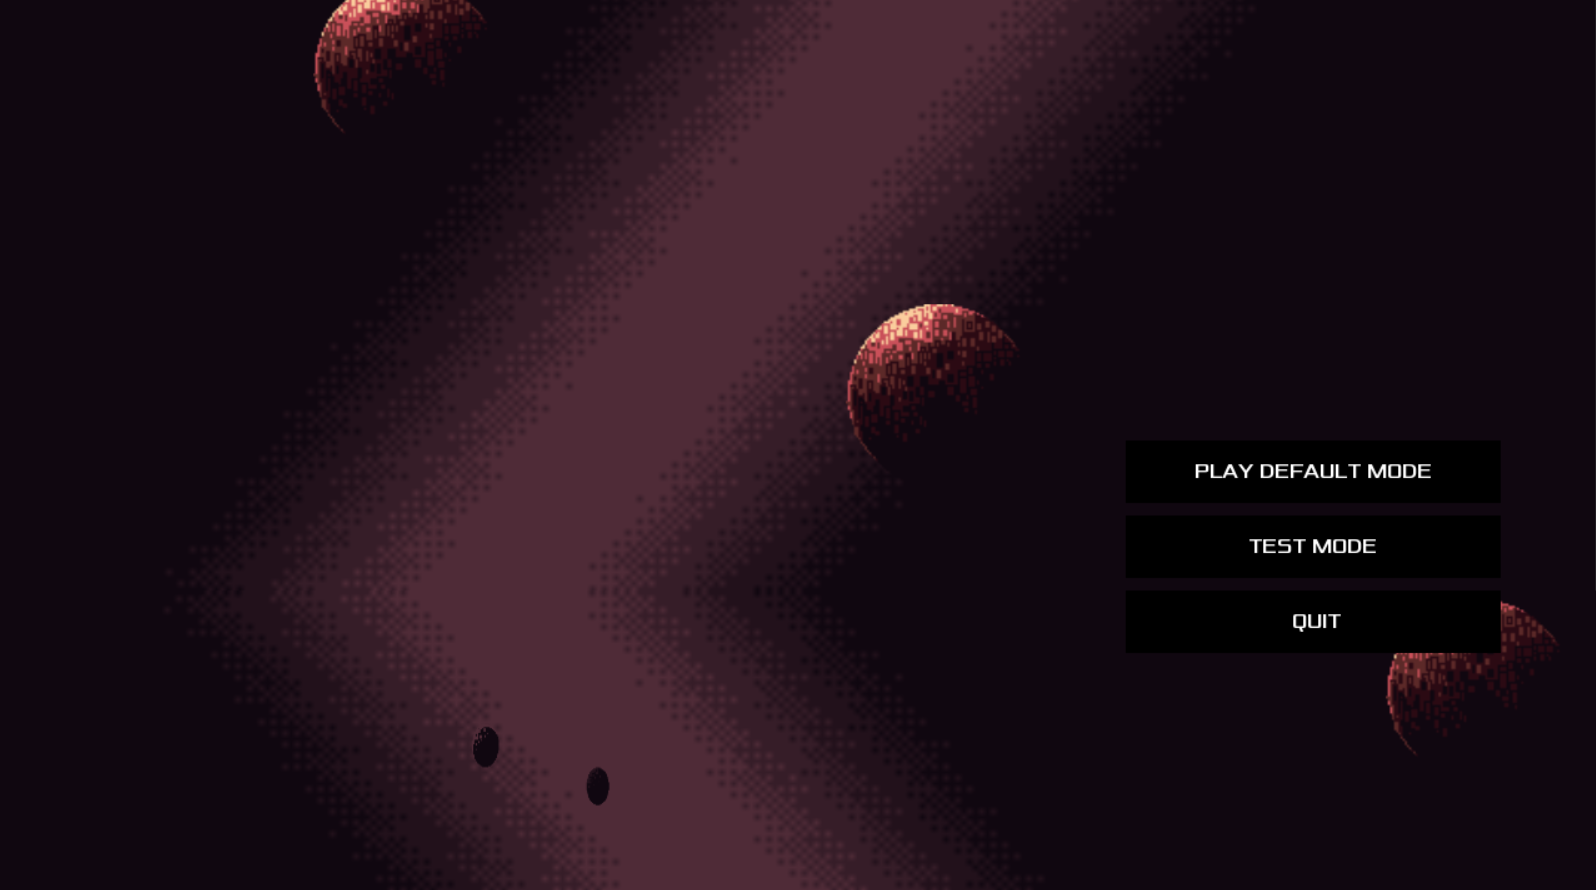
\includegraphics[width=.8\textwidth]{ss/Menu_SS.png}
  \caption{Tela de Teste Space Shooter. Imagem retirada do próprio jogo.\label{fig:tela-de-teste-space-shooter}}
\end{figure}


O menu \textit{Test Mode} permite escolher as configurações necessárias para a execução de um teste, com condições específicas e pré-definidas para obtenção de dados sobre as ondas geradas e o dano total produzido, o menu \textit{Test Mode} de cada jogo encontram-se nas Figuras \ref{fig:td-testes} e  \ref{fig:ss-testes}.

O algoritmo genético foi testado (opção \textit{AI} no menu), em conjunto com opções ingênuas nos dois jogos, posto que foram implementadas para ser comparadas com as ondas geradas pelo algoritmo desenvolvido, em vista de observar se seu desempenho. Assim há opções, apresentadas nas Figuras \ref{fig:td-testes} e \ref{fig:ss-testes} onde as ondas podem ser geradas:
\begin{itemize}
  \item Aleatoriamente - \textit{RANDOM}
  \item Um de cada oponente - \textit{ONE EACH}
  \item Modos "repetição", onde todo inimigo é do mesmo tipo
\end{itemize}

\begin{figure}
  \centering
  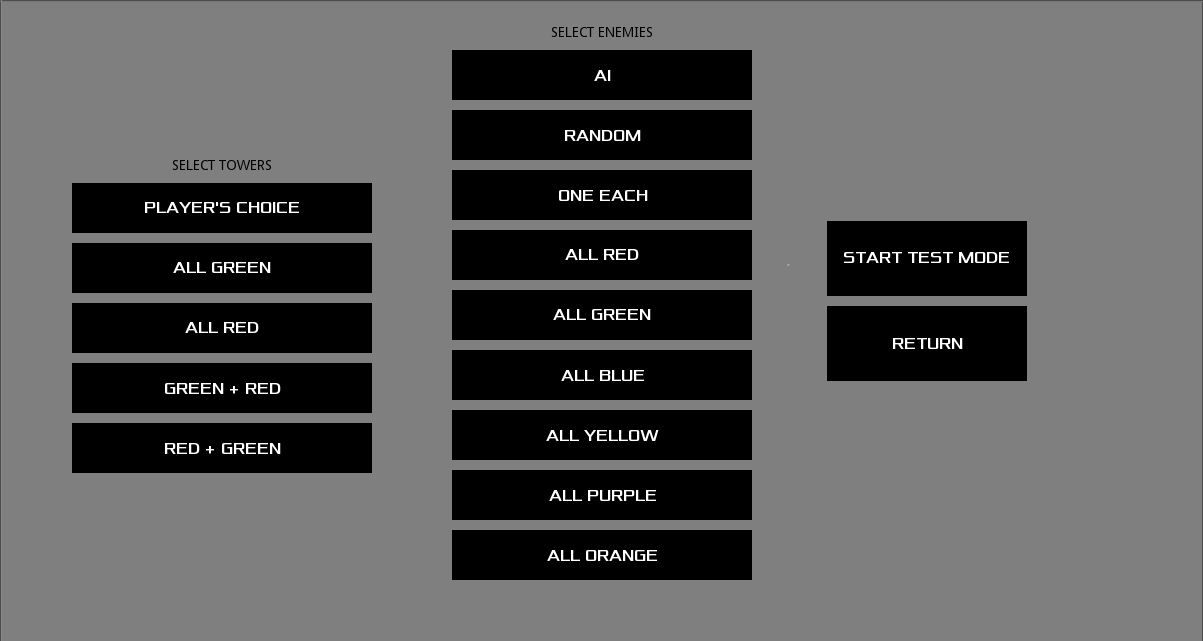
\includegraphics[width=.8\textwidth]{figuras/td/Menu_Escolhas_TESTE_TDD.PNG}
  \caption{Menu de testes Tower Defense. Imagem retirada do próprio jogo.\label{fig:td-testes}}
\end{figure}


\begin{figure}
  \centering
  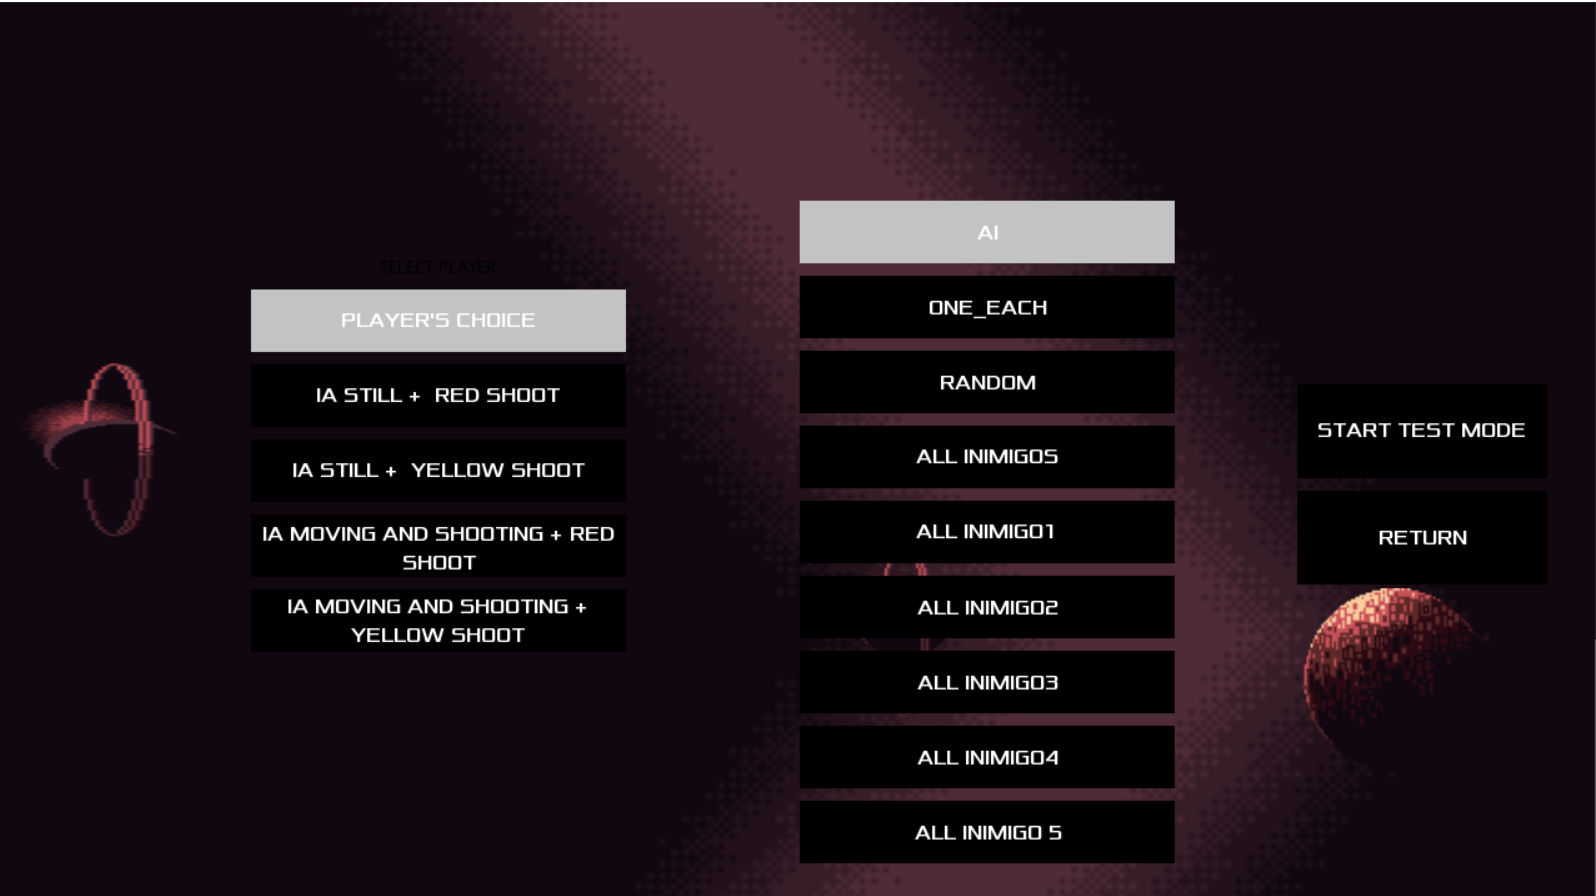
\includegraphics[width=.9\textwidth]{ss/Tela de testes_SS.png}
  \caption{Menu de Testes Space Shooter. Imagem retirada do próprio jogo.\label{fig:ss-testes}}
\end{figure}

\pagebreak

%% ------------------------------------------------------------------------- %%
\subsection{Tower Defense}
\label{sec:mt-td}

No \textit{Tower Defense}, as ondas repetidas enviam 6 inimigos iguais para cada rota norte e sul, um exemplo de uma onda repetida encontra-se na Figura \ref{fig:td-testes-orange} seguindo as rotas que foram já definidas conforme a Figura \ref{fig:td-rota}. Cada onda repetida envia o mesmo tipo de tanque, cujos atributos estam disponíveis na Tabela \ref{tab:tank-dmg2}. O modo \textit{One Each} utiliza os 6 tipos em cada rota; e o \textit{Random} aleatoriza completamente a escolha de tipo e rota, utilizando \textit{RandomNumberGenerator} disponibilizada pela \textit{Godot Engine}. Os modos \textit{Random} e \textit{One Each} podem ser vistos nas Figuras \ref{fig:tdd-testes} e \ref{fig:td-testes-one-each}. 


\begin{figure}
  \centering
  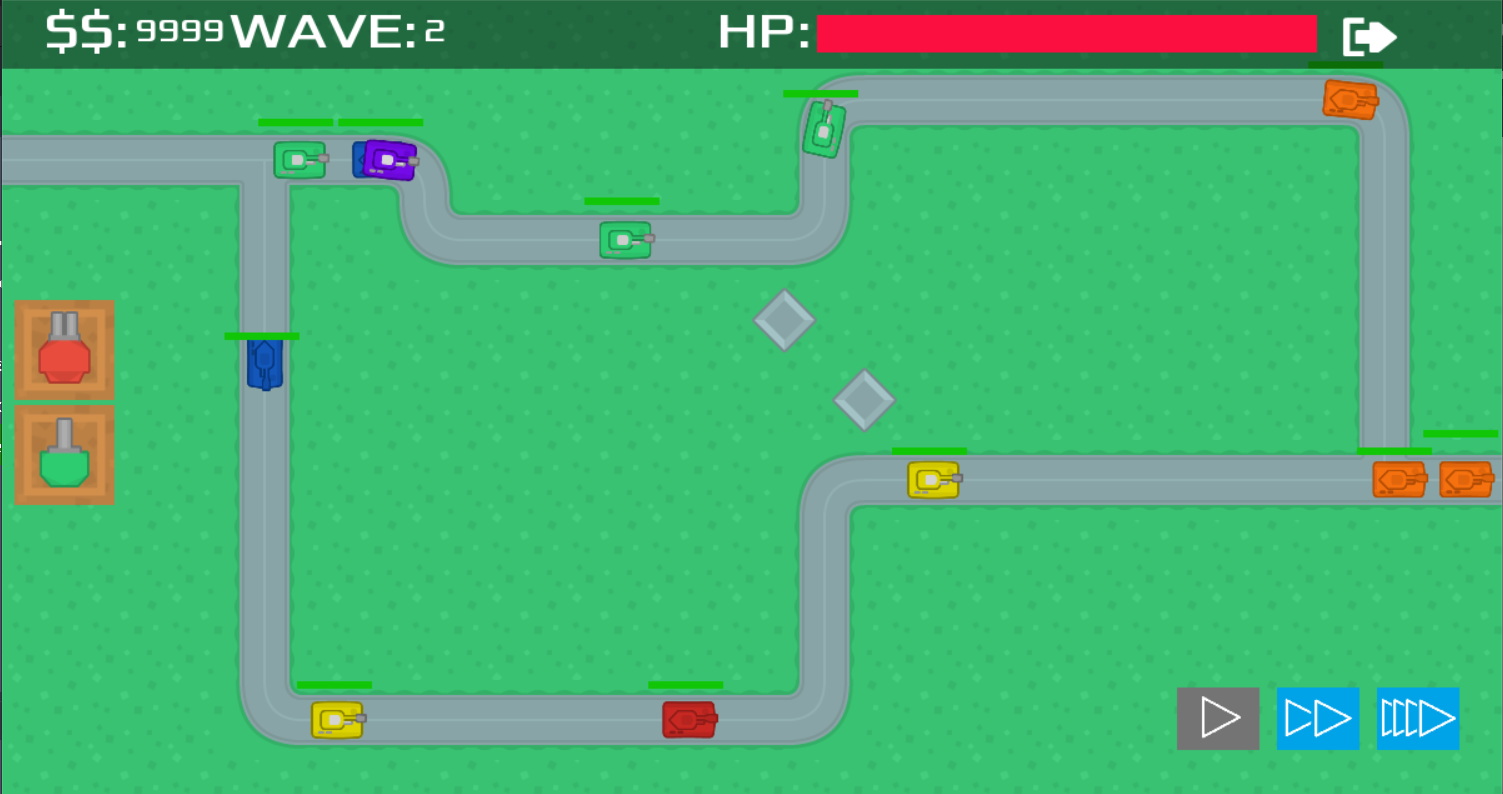
\includegraphics[width=.9\textwidth]{td/Random Mode_TDD Teste.PNG}
  \caption{Escolha Random em tower defense. Imagem retirada do próprio jogo.\label{fig:tdd-testes}}
\end{figure}


\begin{figure}
  \centering
  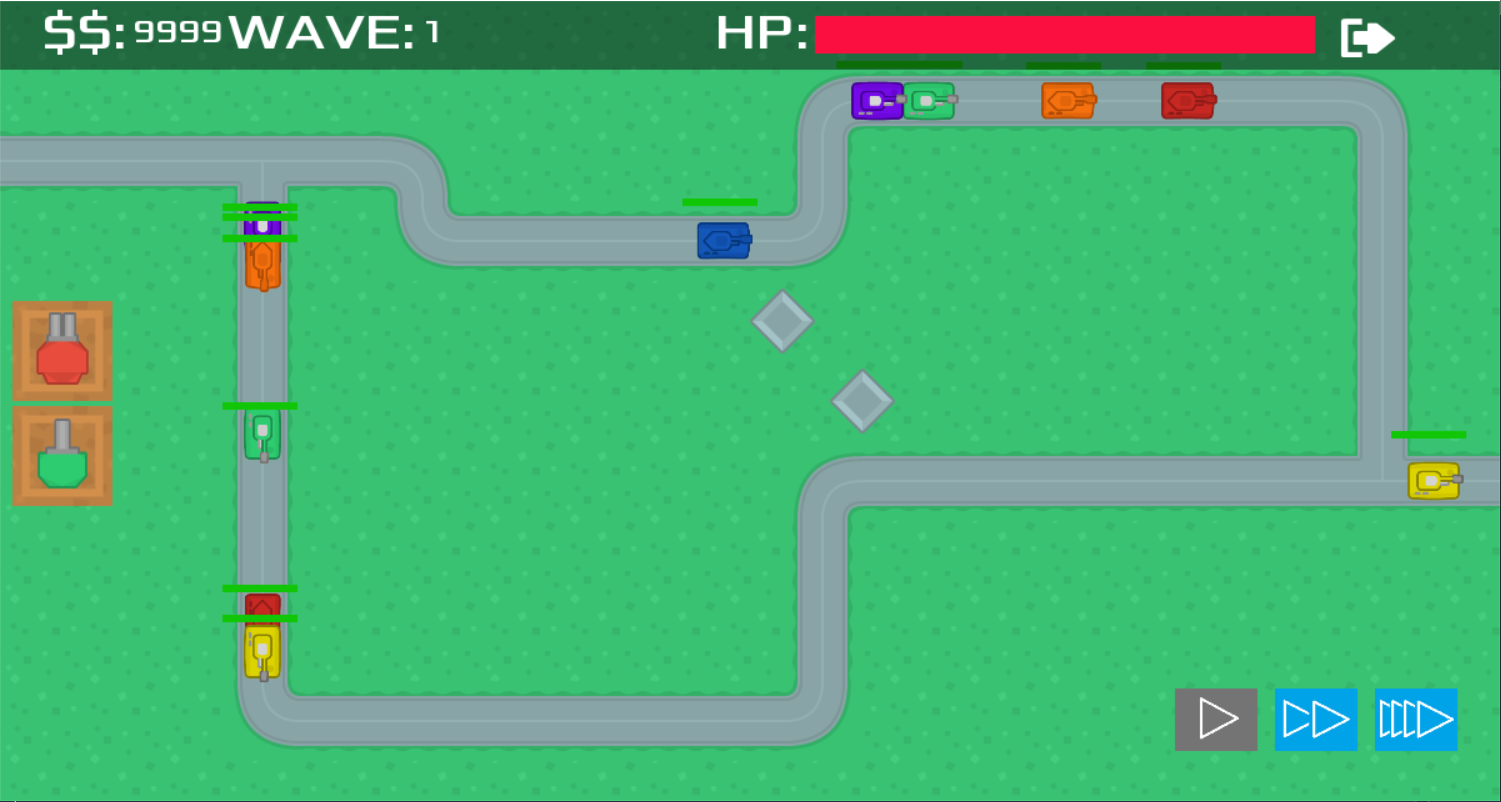
\includegraphics[width=.9\textwidth]{td/Exempleo TDD One EACH.PNG}
  \caption{Escolha One Each no Tower Defense. Imagem retirada do próprio jogo.\label{fig:td-testes-one-each}}
\end{figure}


\begin{figure}
  \centering
  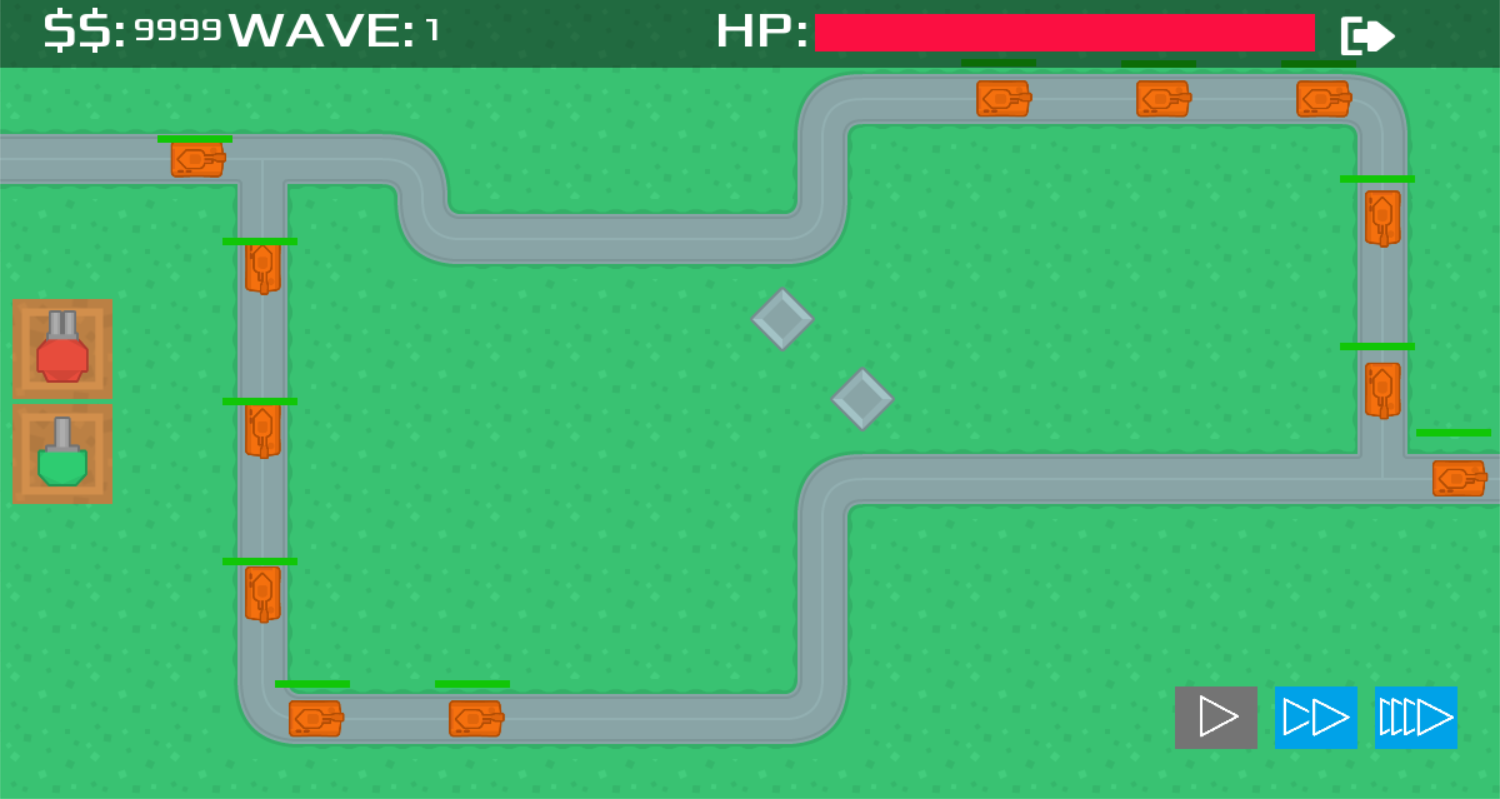
\includegraphics[width=.9\textwidth]{td/Tdd_All_orange.PNG}
  \caption{Opção All Orange. Imagem retirada do próprio jogo.\label{fig:td-testes-orange}}
\end{figure}

\pagebreak

Para uniformizar o comportamento do jogador, as torres foram configuradas para melhor controle dos testes, posicionadas duas por rota, onde o alcance das mesmas fica restrito a somente seu caminho, de maneira a alcançar um balanço entre eliminação e sobrevivência de alguns oponentes, visto as torres terem diferentes valores atribuídos com relação a dano e alcance, presentes na Tabela \ref{tab:dados_torres2}. Assim são geradas 4 configurações de teste, demonstradas nas Figuras \ref{fig:td-teste-all-green}, \ref{fig:tdd-teste-all-red}, \ref{fig:tdd-teste-greenred}, \ref{fig:td-teste-red-green}.

\begin{table}
\caption{Dano das torres no Tower Defense.\label{tab:dados_torres2}}
\begin{tabular}{c|ccc}

             & velocidade de tiro  & dano & alcance\\ \hline
Torre Verde   & 55     & 25     &  350 \\
Torre Vermelha     & 70     & 15     &  550       

\end{tabular}
\end{table}


\begin{table}
\caption{Dano de cada tanque no Tower Defense}
\begin{tabular}{c|cc}
            & velocidade & dano   \\ \hline
tank blue   & 55    & 55         \\
tank green  & 70    & 45         \\
tank red    & 80    & 15          \\
tank orange & 120   & 5           \\
tank purple & 90    & 15          \\
tank yellow & 150   & 5           
\end{tabular}
\label{tab:tank-dmg2}
\end{table}

\pagebreak

\begin{figure}
  \centering
  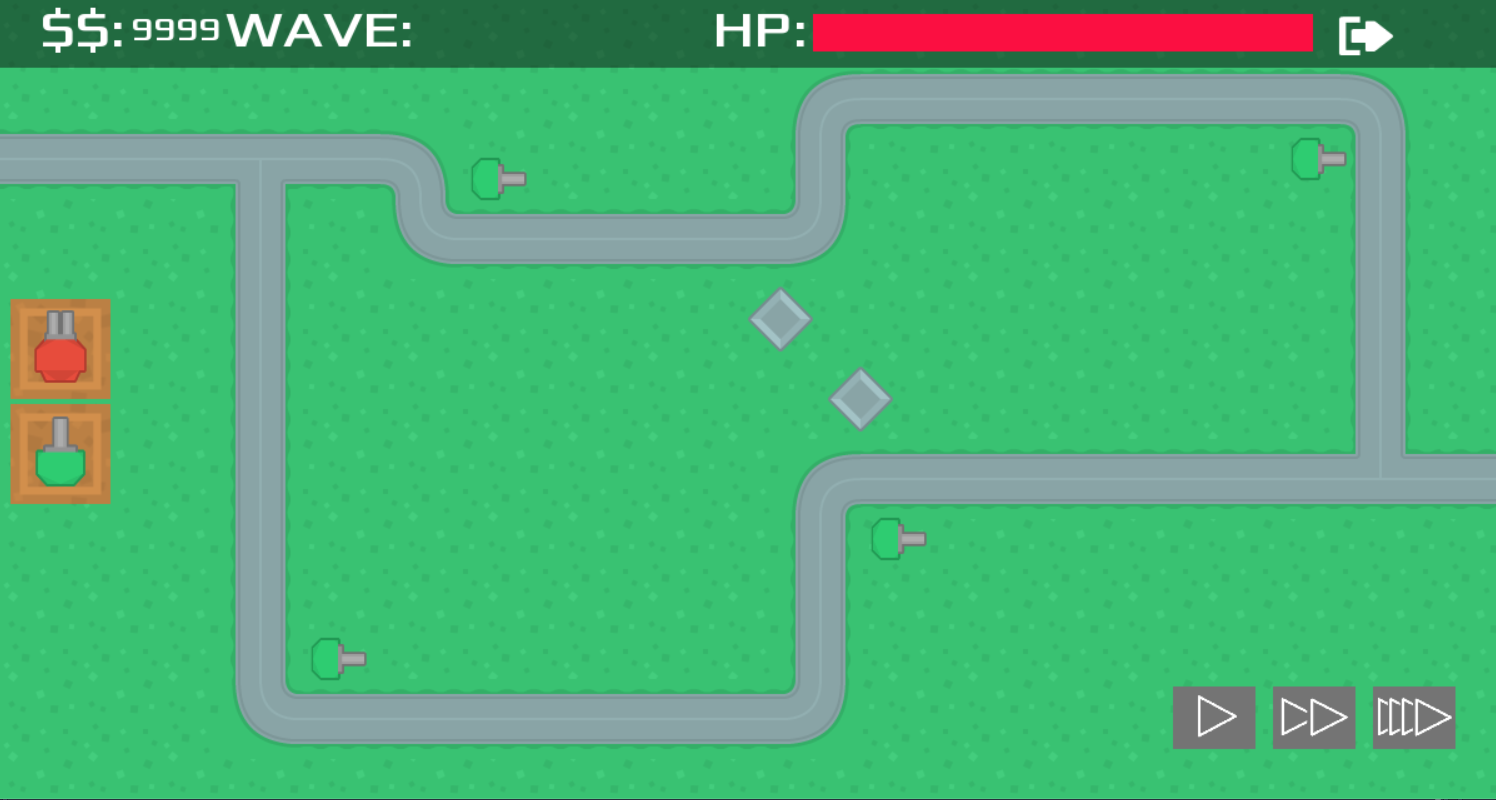
\includegraphics[width=.9\textwidth]{td/Tdd_all_green_teste.png}
  \caption{Teste de torres verdes\label{fig:td-teste-all-green}}
\end{figure}

\begin{figure}
  \centering
  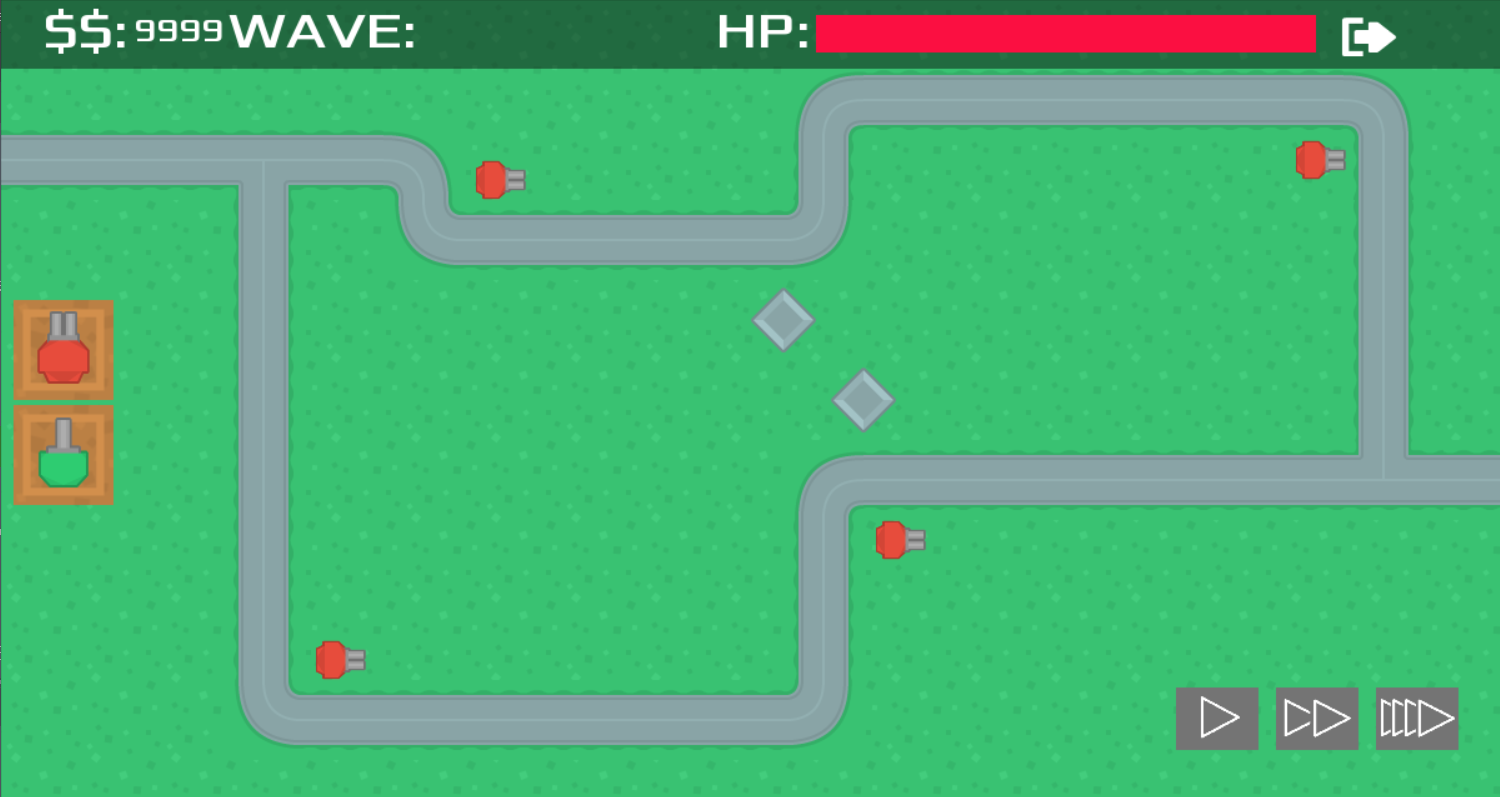
\includegraphics[width=.9\textwidth]{td/ALL RED TDD.png}
  \caption{Teste de torres vermelhas\label{fig:tdd-teste-all-red}}
\end{figure}

\begin{figure}
  \centering
  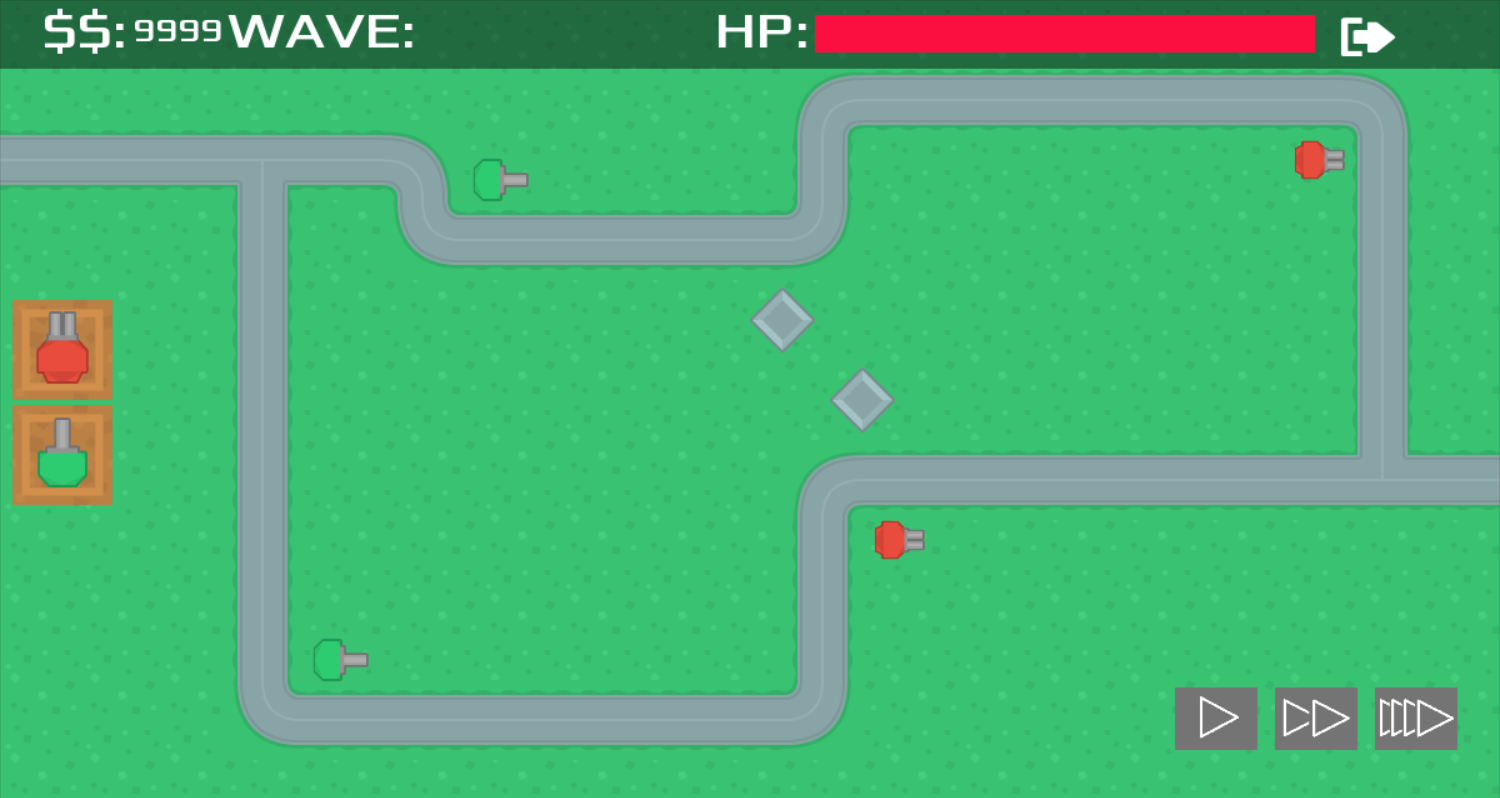
\includegraphics[width=.9\textwidth]{td/Green_Red_TDD.png}
  \caption{Teste de torres verdes com vermelhas\label{fig:tdd-teste-greenred}}
\end{figure}

\begin{figure}
  \centering
  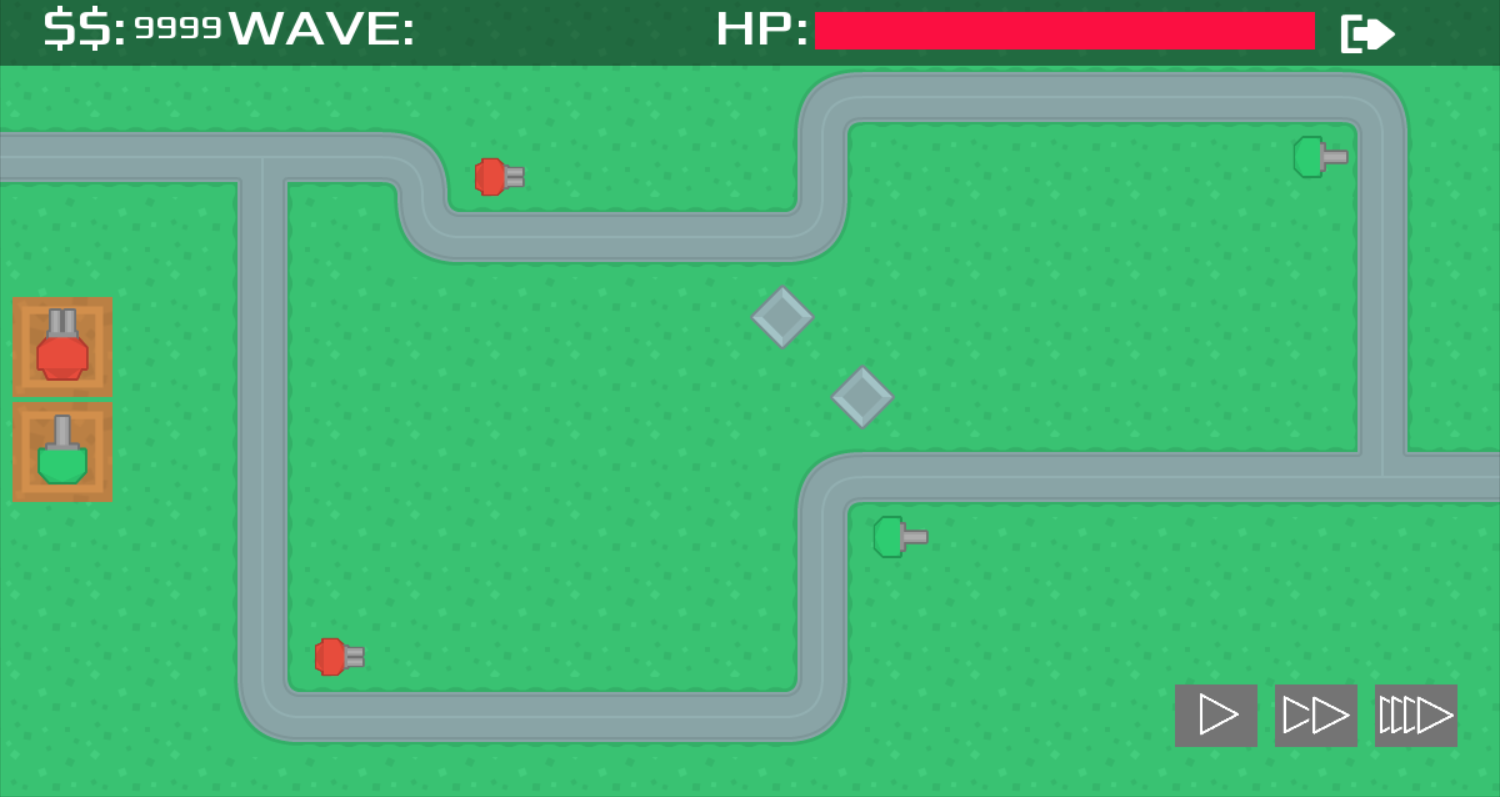
\includegraphics[width=.9\textwidth]{td/RED_GREEN TDD.png}
  \caption{Teste de torres vermelhas com verdes\label{fig:td-teste-red-green}}
\end{figure}

\newpage
%% ------------------------------------------------------------------------- %%
\subsection{Space Shooter}
\label{sec:mt-ss}

O \textit{Space Shooter} foi configurado de maneira próxima do \textit{Tower Defense}, mas foi preservada a capacidade dos asteroides aparecerem em locais aleatórios entre os 6 possíveis do jogo, exceto quando a IA está gerando os inimigos, onde o algoritmo busca o melhor \textit{spawn}. As naves foram alteradas para efetivamente jogarem a partida; com um nó \textit{Area2D} ao seu redor para detecção e ataque contra o primeiro inimigo que colidir contra o nó, conforme a Figura \ref{fig:ss-area}; e com a implementação de uma opção de movimentação, visto a Figura \ref{fig:ss-move}, permitindo testes com uma nave estática no centro da tela, e com movimentação lateral, de lado a lado, pausando nas extremidades.

\begin{figure}
  \centering
  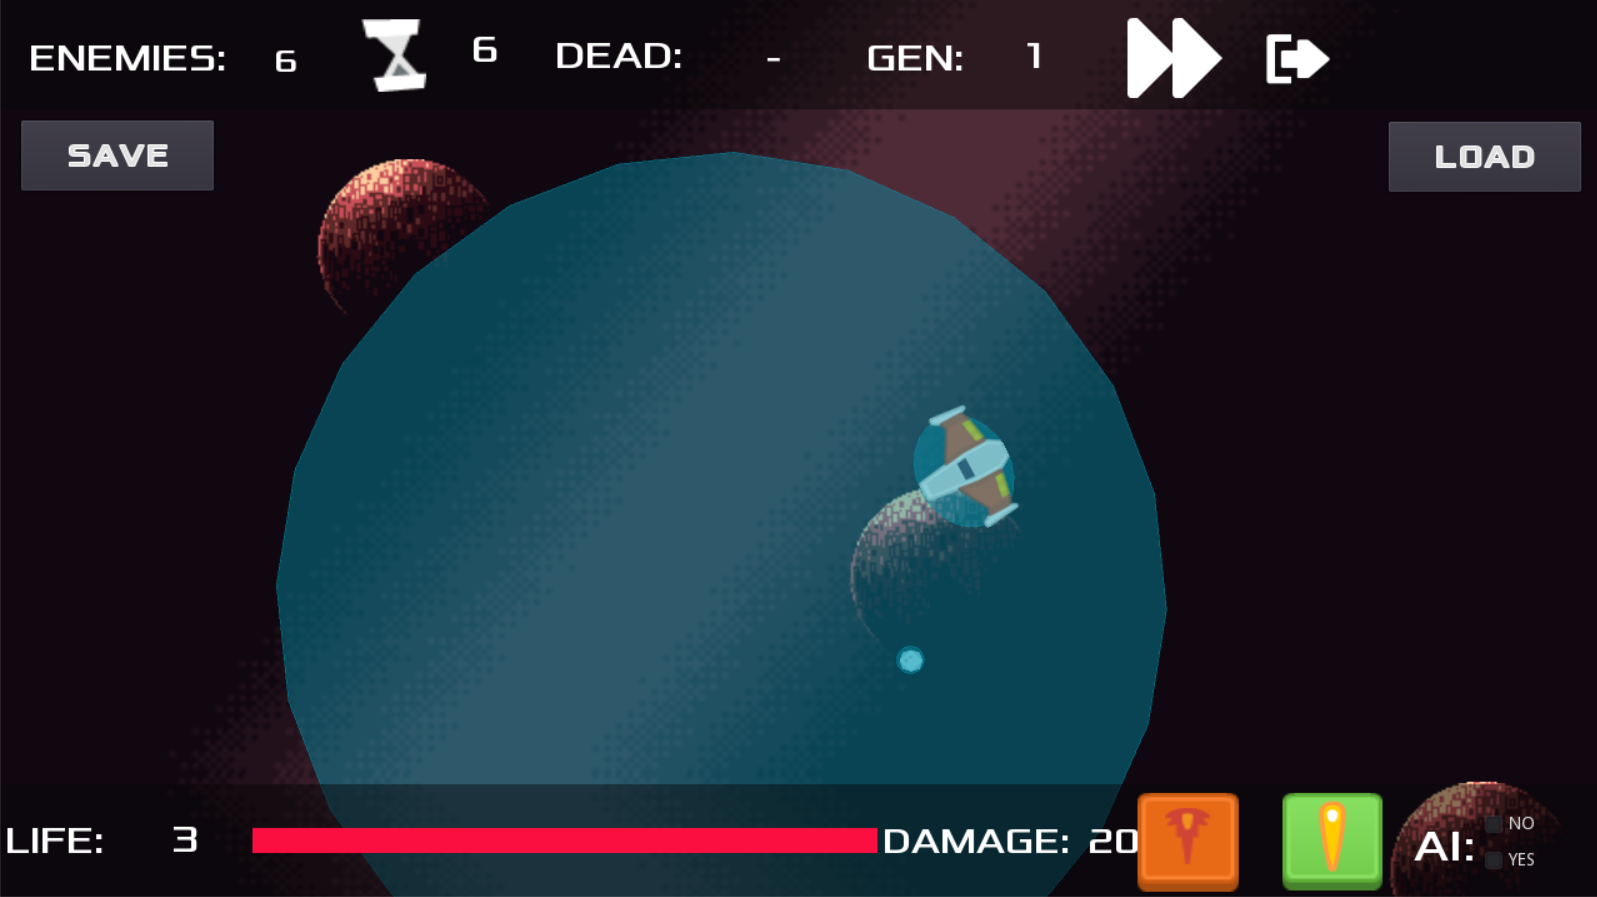
\includegraphics[width=.9\textwidth]{ss/Area de deteccao_Player_IA_jogo_exemplo.png}
  \caption{Área de detecção da nave em um modo de teste. Imagem retirada do próprio jogo.\label{fig:ss-area}}
\end{figure}

\begin{figure}
  \centering
  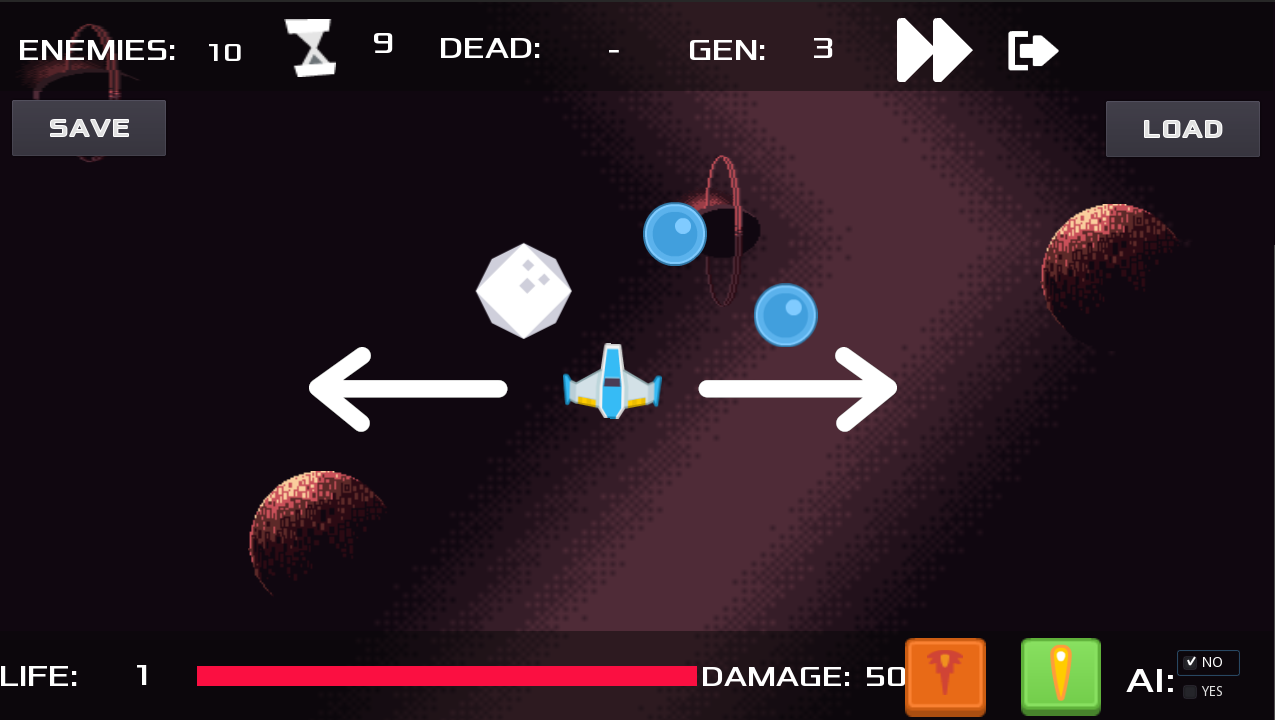
\includegraphics[width=.9\textwidth]{ss/ss_move.png}
  \caption{Movimentação da nave em um modo de teste. Imagem retirada do jogo e editada.\label{fig:ss-move}}
\end{figure}

\pagebreak

As opções dos inimigos são semelhantes ao \textit{Tower Defense}, com ondas sempre com os mesmos inimigos, ou um de cada, ou escolhendo aleatoriamente através do \textit{RandomNumberGenerator} da \textit{engine}. Reiterando que nestes casos o \textit{spawn} dos asteroides ocorre em qualquer um dos 6 locais disponíveis na Figura \ref{fig:ss-positions} escolhidos de maneira aleatória pelo jogo.